
\section{Evaluation}
\label{sec:evaluation}

We evaluate the design of Legion's static and dynamic semantics on four criteria:
expressivity (can real applications be written---Section~\ref{subsec:expressivity}),
overhead  (what are the dynamic checking costs---Section~\ref{subsec:overhead}),
scalability (can it enable hierarchical scheduling---Section~\ref{subsec:scalability}),
and performance  (does the performance increase from relaxed coherence modes 
warrant the increased semantic complexity---Section~\ref{subsec:relaxedperf}).
%Our evaluation uses a prototype implementation of the Legion language and programming model.
Our prototype implementation has two components: a type checker
for the language of Section~\ref{sec:legioncore} and a C++ runtime library
for executing programs written in the Legion programming model.  All experiments
are conducted on the Keeneland supercomputer\cite{Keeneland}.  Each node of Keeneland
consists of two Xeon 5660 CPUs, three Tesla M2090 GPUs, and 24 GB of DRAM.  Nodes
are connected by a QDR Infiniband interconnect.

\subsection{Expressivity}
\label{subsec:expressivity}
We evaluate Legion on three real-world applications.  To qualitatively gauge the 
expressivity of Legion, we introduce these applications
by describing features used in their implementations.
The Circuit example was already covered in detail in Section~\ref{sec:example}.

%\subsubsection{Circuit Simulation}
%\label{subsec:circuit}
%Circuit simulates the wires of a large integrated circuit.
% using an RLC model.  
%The computation consists of three phases for each time step: compute the current in each wire using
%an iterative model, updated the charge in each node, and compute the voltage of each node.
%The primary data structure is a large irregular graph, which is
%dynamically partitioned into pieces to enable parallel simulation.
%Our implementation creates separate regions for the wires and
%nodes,  which are recursively partitioned into
%subregions for pieces of the graph.  The node region is partitioned an additional way to 
%describe the sets of ghost nodes required for each piece.  
%The information about each piece of the graph is stored
%in a region relationship that remembers the disjointness information of each piece
%from other pieces.  The tasks for the three phases of the computation use different combinations of
%read, write, and reduce privileges as well as exclusive and simultaneous coherence.

%\subsubsection{Fluid Simulation}
%\label{subsec:fluid}
Fluid is a distributed memory version of the {\tt fluidanimate} benchmark from the PARSEC 
suite\cite{bienia11benchmarking}.  Fluid simulates the flow of an incompressible fluid
using particles that move within a regular grid of cells.  To perform operations in 
parallel the array of cells is partitioned.  Unlike
Circuit, Fluid creates and partitions regions before
allocating cells in them. 
%(i.e., partition-then-allocate).  
Another difference is that Fluid
maintains separate regions for ghost cells rather using multiple partitions of
the regions containing shared data.  Region relationships are used to capture
which regions are required for each grid.

%\subsubsection{Adaptive Mesh Refinement}
%\label{subsec:amr}

The third application is a Legion port of an adaptive mesh refinement (AMR) benchmark 
from BoxLib \cite{BoxLib}.  The algorithm solves the two
dimensional heat diffusion equation on a grid of cells using three levels of refinement with sub-refinements
randomly placed on the surface.  
%For each time step in the application, cells at the boundary of
%a refinement are interpolated from cells at a coarser level of refinement, energy fluxes between
%cells are computed, energy is transferred, and cells at a coarser level of refinement are restricted
%to the values of refined cells.  
Every level of refinement uses a separate region, which is partitioned several ways to support multiple views of
the cells.  One partitioning separates cells into pieces that can be updated in
parallel.  Additional partitions are created for viewing data from coarser and finer levels of
the simulation.  Two types of region relationships are created: one describes pieces at 
each level of refinement, and another describes relationships between pieces at different
levels of refinement.  
%These region relationships capture both intra- and inter-level disjointness information.  
The dynamic nature of AMR requires that regions be created and partitioned at runtime.  
%The many ways in which cells are used also requires multiple simultaneous
%partitions of regions.

%These applications directly demonstrate the need to for multiple, dynamic partitions
%of program data.
%These applications demonstrate Legion is capable of 
%expressing real applications with both regular (Fluid, AMR) and 
%irregular (Circuit) pointer data structures.

Dynamically creating and partitioning regions at runtime is crucial to Legion's
ability to handle applications that make runtime decisions about data organization (AMR).  
% FIXME
% I've deemphasized the point about allocate-then-partition vs. partition-then-allocate.
% If we want to put it back in it needs to be go in multiple places, not just here.
%Legion is able to capture both allocate-then-partition (Circuit) and partition-then-allocate (Fluid) algorithms. 
Having multiple partitions of regions is necessary for describing the many ways 
that data can be accessed (Circuit, AMR).  All the types of privileges and coherence 
are needed in some application;  region relationships
are used in all applications.   Finally, all applications introduce aliasing of
data through both multi-colorings or having multiple partitions.  Our implementations of
these applications both type check and execute, proving that our type system is
sufficiently expressive to handle real-world applications.
% written in the Legion programming model.
%, region relationships convey disjointness information.
% despite
%regions being a first-class feature that cannot be fully tracked statically.

\subsection{Checking Overhead}
\label{subsec:overhead}
The first Legion implementation consisted of a C++ library of Legion primitives
\cite{Legion12} with no checking of region memory accesses.  
When using this system we frequently encountered memory corruption due to
illegal region accesses caused by application bugs.
In many cases, this corruption occurred between nodes in the cluster or on 
GPUs, environments for which debugging tools are primitive at best.
%  Finding these bugs required either multiple {\tt gdb} sessions 
%for observing execution on different nodes simultaneously or using {\tt printf} for debugging on
%GPUs.  
To locate the application bugs causing these illegal accesses, we initially added 
dynamic checks on  all region accesses for both CPUs and GPUs which  
added considerable runtime overhead.  
To preserve the benefit of checking every access without the cost of dynamic checks, we implemented the type, privilege, and coherence checker we have described. 
We then rewrote the applications in this language and type checked them, at which point the
dynamic region access checks could be safely elided.

%\begin{figure}
%\subfigure[48 Piece Data Set]
%{
%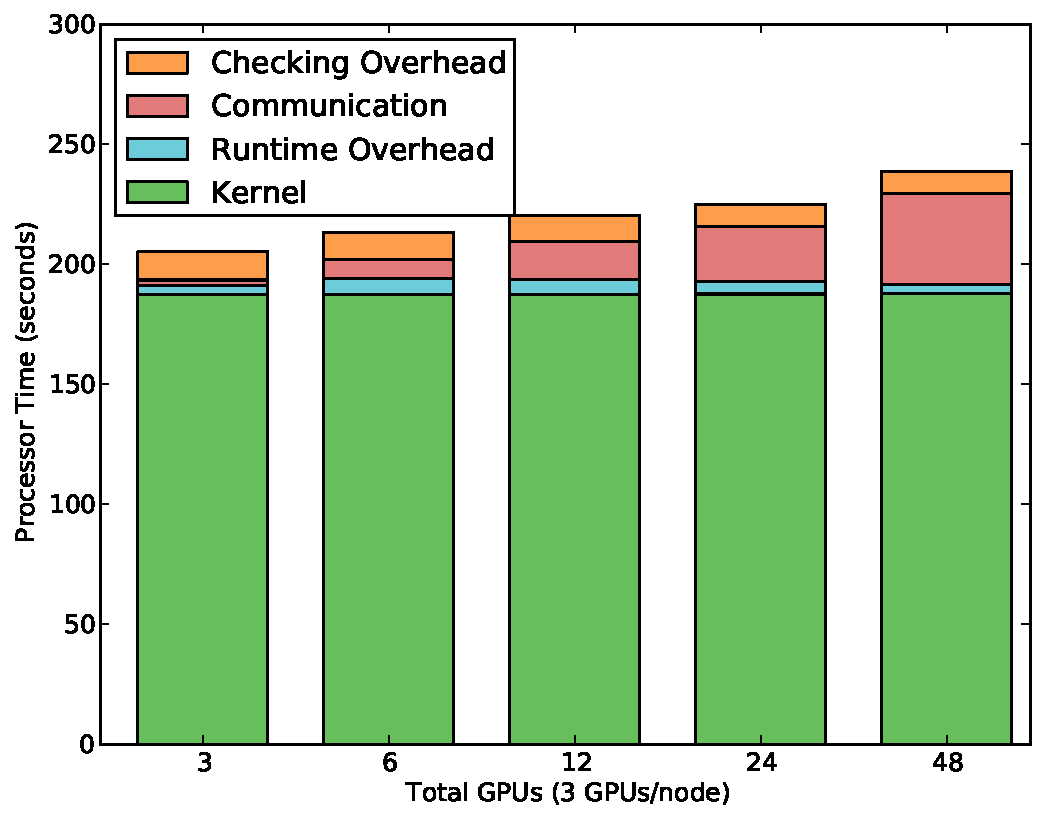
\includegraphics[scale=0.4]{figs/circuit_48_popl.pdf}
%\label{fig:ckt48}
%}
%\subfigure[96 Piece Data Set]
%{
%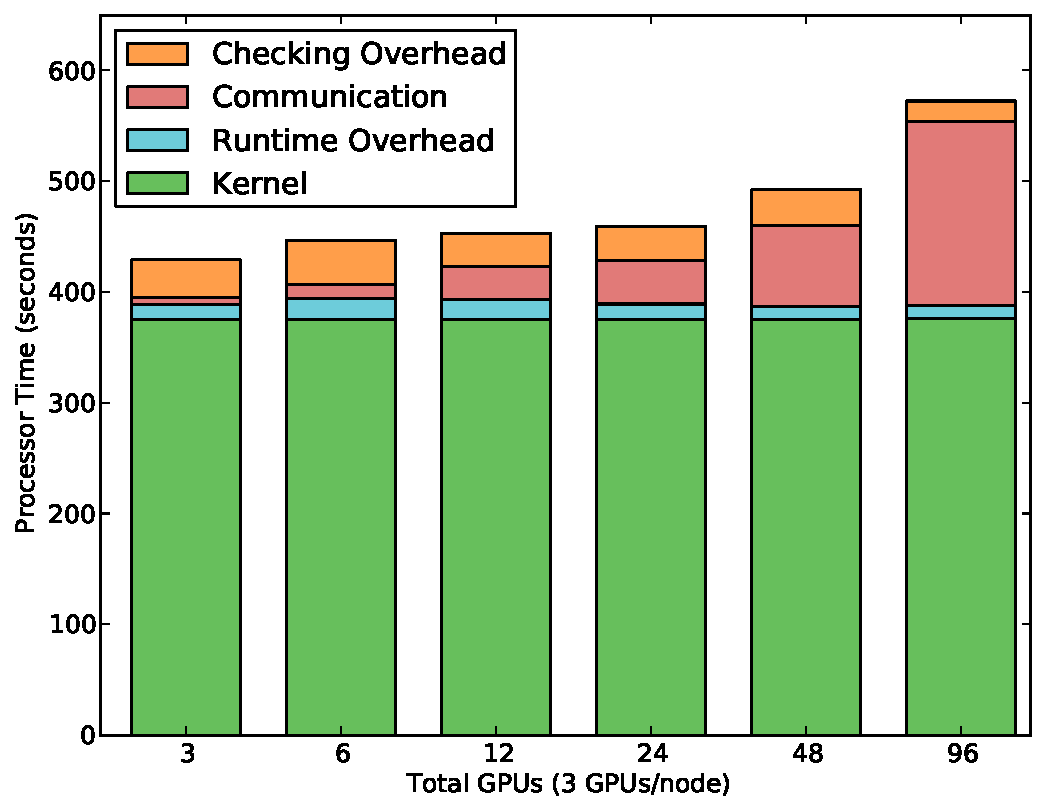
\includegraphics[scale=0.4]{figs/circuit_96_popl.pdf}
%\label{fig:ckt96}
%}
%\caption{Checking overhead of the Circuit simulation.\label{fig:ckt_overhead}}
%\end{figure}

\begin{figure}
\begin{center}
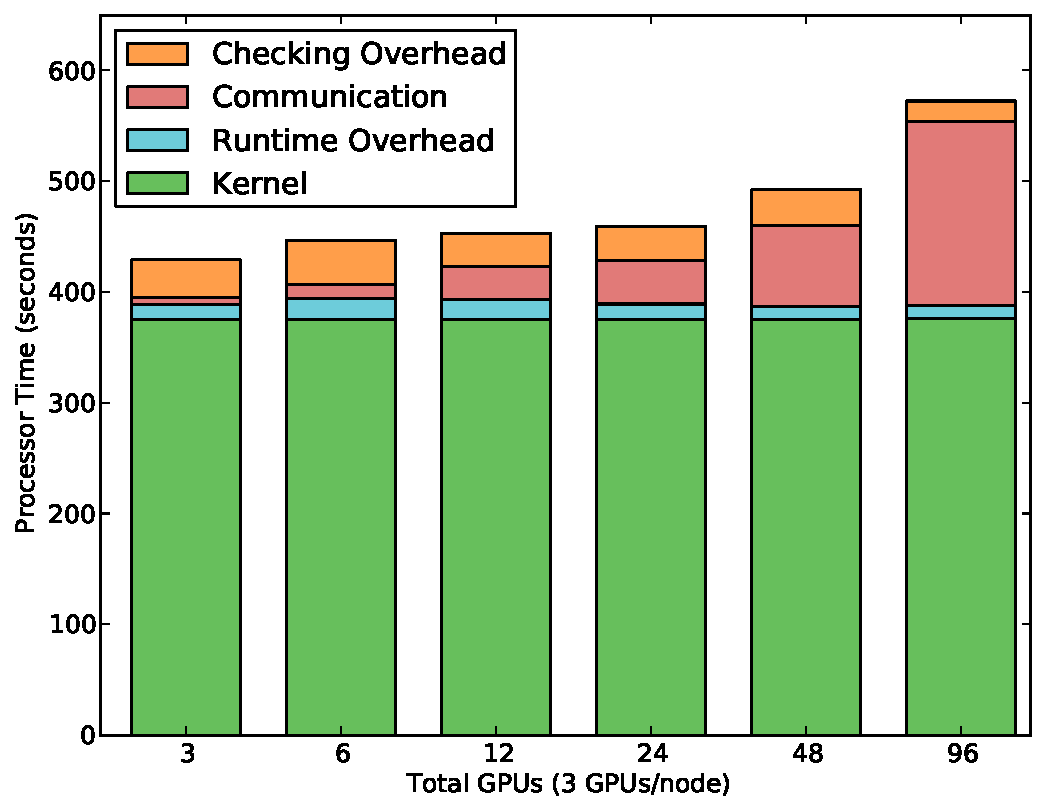
\includegraphics[scale=0.30]{figs/circuit_96_popl.pdf}
\end{center}
\vspace{-2mm}
\caption{Overhead for the Circuit simulation with 96 total pieces.\label{fig:ckt_overhead}}
\vspace{-5mm}
\end{figure}

\begin{figure}
\begin{center}
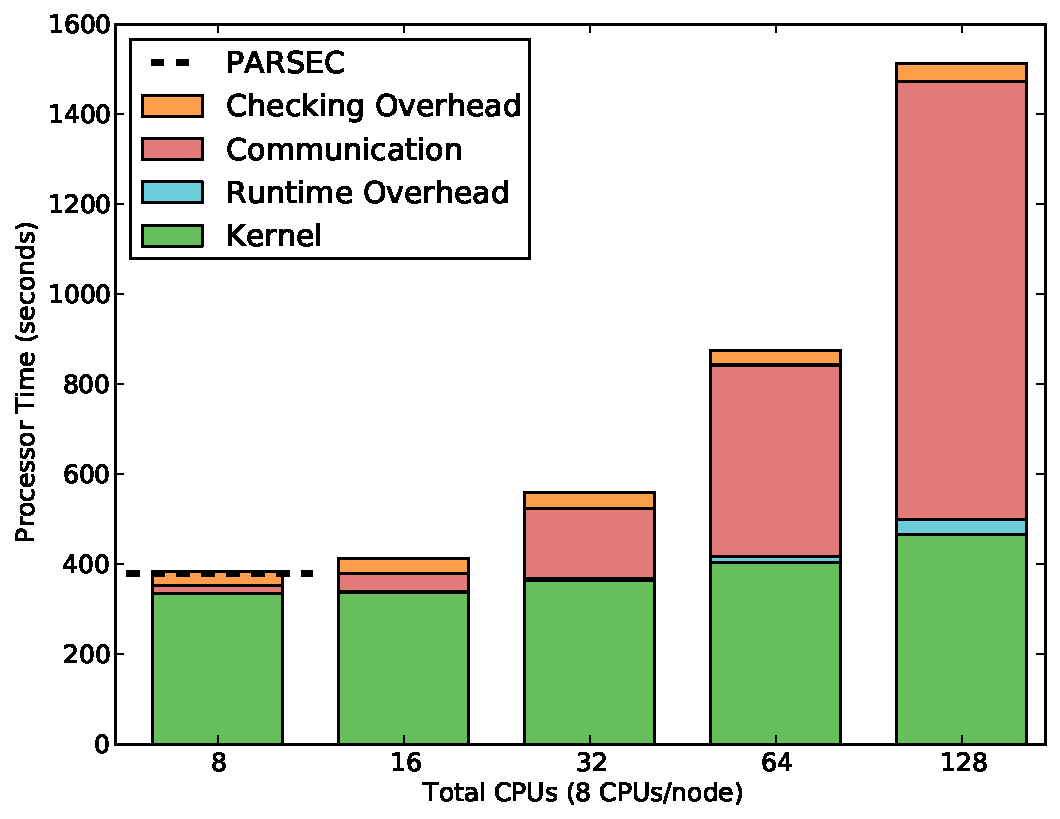
\includegraphics[scale=0.30]{figs/fluid_19200_popl.pdf}
\end{center}
\vspace{-2mm}
\caption{Overhead for the Fluid simulation with 19200 cells.\label{fig:fluid_overhead}}
\vspace{-5mm}
\end{figure}

Figures~\ref{fig:ckt_overhead}, \ref{fig:fluid_overhead}, and \ref{fig:amr_overhead} show 
the total time spent by all CPUs and GPUs in each phase of the application.  The topmost
component of each bar shows the overhead added by the dynamic checks.  In 
each figure the problem size stays the same as the number of processors increases
(strong scaling).  Figure~\ref{fig:amr_overhead} includes multiple problem sizes to show
how overhead is affected by changing problem size (weak scaling).  For cases where there
is an existing implementation to compare against we have included a dotted line indicating
baseline performance.  In a few cases (Figures~\ref{fig:fluid_overhead} and 
\ref{fig:amr4096}), the checking overhead is the difference
between better and worse performance than the baseline.  The overall
performance relative to the baseline implementations is discussed in \cite{Legion12}.

\begin{figure}
\begin{center}
\subfigure[4096 cells per dimension]
{
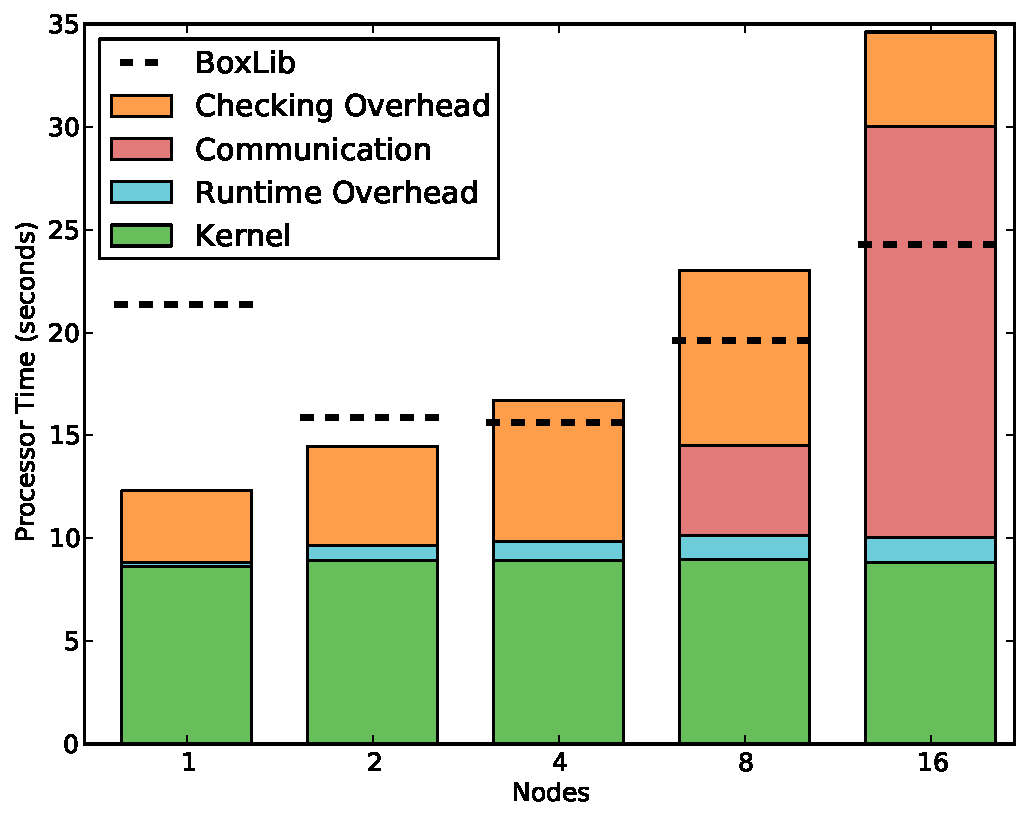
\includegraphics[scale=0.30]{figs/amr_4096_popl.pdf}
\label{fig:amr4096}
}
\subfigure[8192 cells per dimension]
{
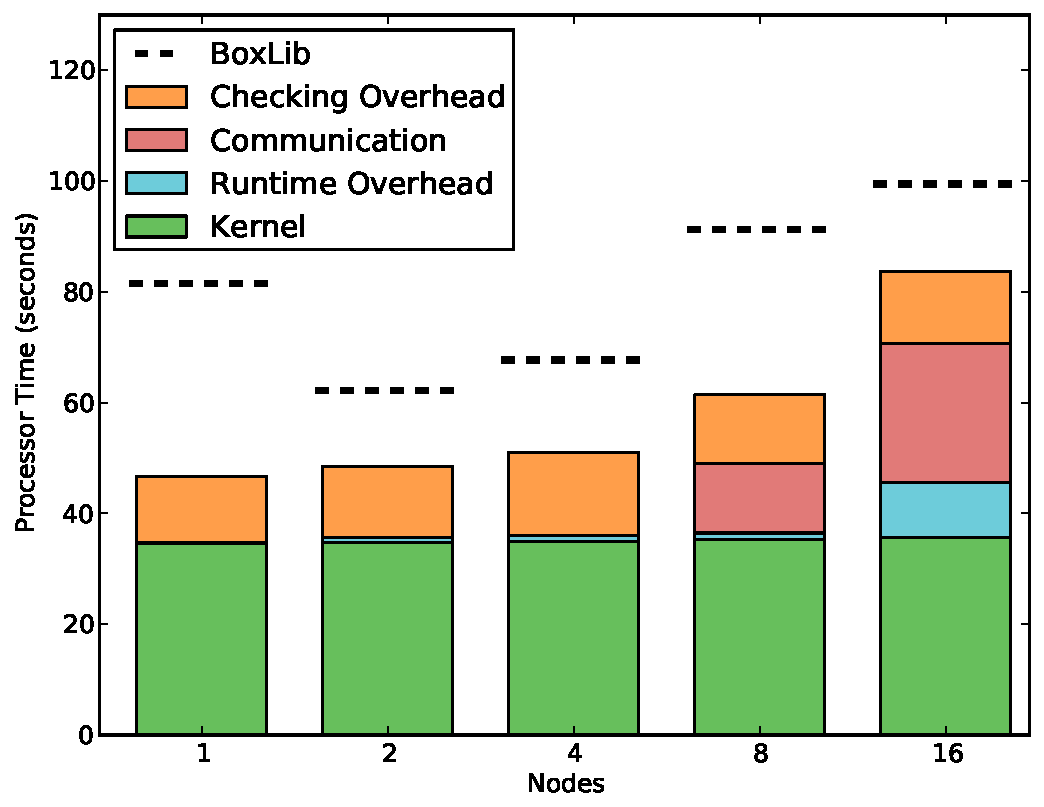
\includegraphics[scale=0.30]{figs/amr_8192_popl.pdf}
\label{fig:amr8192}
}
\subfigure[16384 cells per dimension]
{
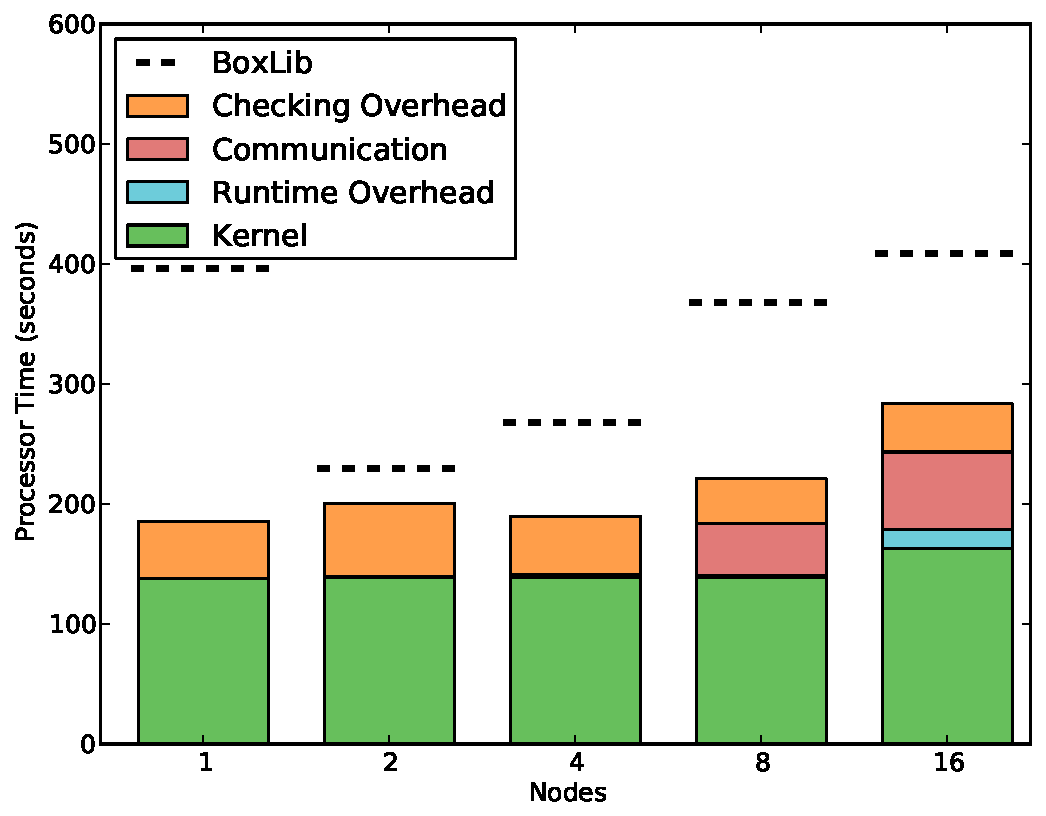
\includegraphics[scale=0.30]{figs/amr_16384_popl.pdf}
\label{fig:amr16384}
}
\end{center}
\vspace{-2mm}
\caption{Overhead for the AMR application.\label{fig:amr_overhead}}
\vspace{-8mm}
\end{figure}

In addition to total processor overhead, we also measured performance gain from eliding checks in 
terms of wall-clock time.  Since most region accesses occur in leaf tasks, the checks parallelize 
well.  Wall-clock performance gains from eliding memory checks ranged from 1-10\%, 1-15\%, 
and 2-71\% for Circuit, Fluid, and AMR respectively.  Performance gains for AMR were larger than
the other applications because AMR was already memory bound and the additional checks intensified
memory pressure.  For the GPU kernels in the Circuit application checking required up to 8 additional 
registers per thread.  While the GPU kernels in Circuit were not bound by 
available on-chip memory, kernels that are would be susceptible to extreme performance 
degradation due to the extra registers required for checking.  We also measured the overhead
of the dynamic checks associated with checking task call privileges but found them to be negligible,
demonstrating that runtime non-interference checks are inexpensive in Legion.
% relative to the overhead of region access checks.

\subsection{Scalability}
\label{subsec:scalability}
%The scalability of Legion derives directly from Theorem~\ref{thm:hiersched}.  This 
%theorem proves it is safe for the runtime to only perform dependence checks between two
%tasks that share the same immediate parent task instead of having to consider all
%possible interactions with other tasks anywhere in the system.  Since all tasks that
%share the same immediate parent are all created on the node where the parent is executing,
%all dependence checks and scheduling decisions can be performed locally with no inter-processor communication.  
%Without this property the runtime would be forced to inform all other processors in the system 
%of every task that it launches using expensive broadcasts. 

Figures~\ref{fig:ckt_overhead}, \ref{fig:fluid_overhead}, and \ref{fig:amr_overhead} show that
the overhead of the Legion runtime is always less than 7\% of the total execution time
of the applications.  In some applications communication does not scale well, but this is
a result of the algorithm required by the application, not the Legion runtime.
Even in the case of the Circuit application, which exhibits quadratic communication scaling, the Legion
runtime is able to achieve a 62.5X speedup on 96 GPUs over a hand-coded single GPU implementation\cite{Legion12}.

\begin{figure}
\begin{center}
\subfigure[48 Piece Problem Size]
{
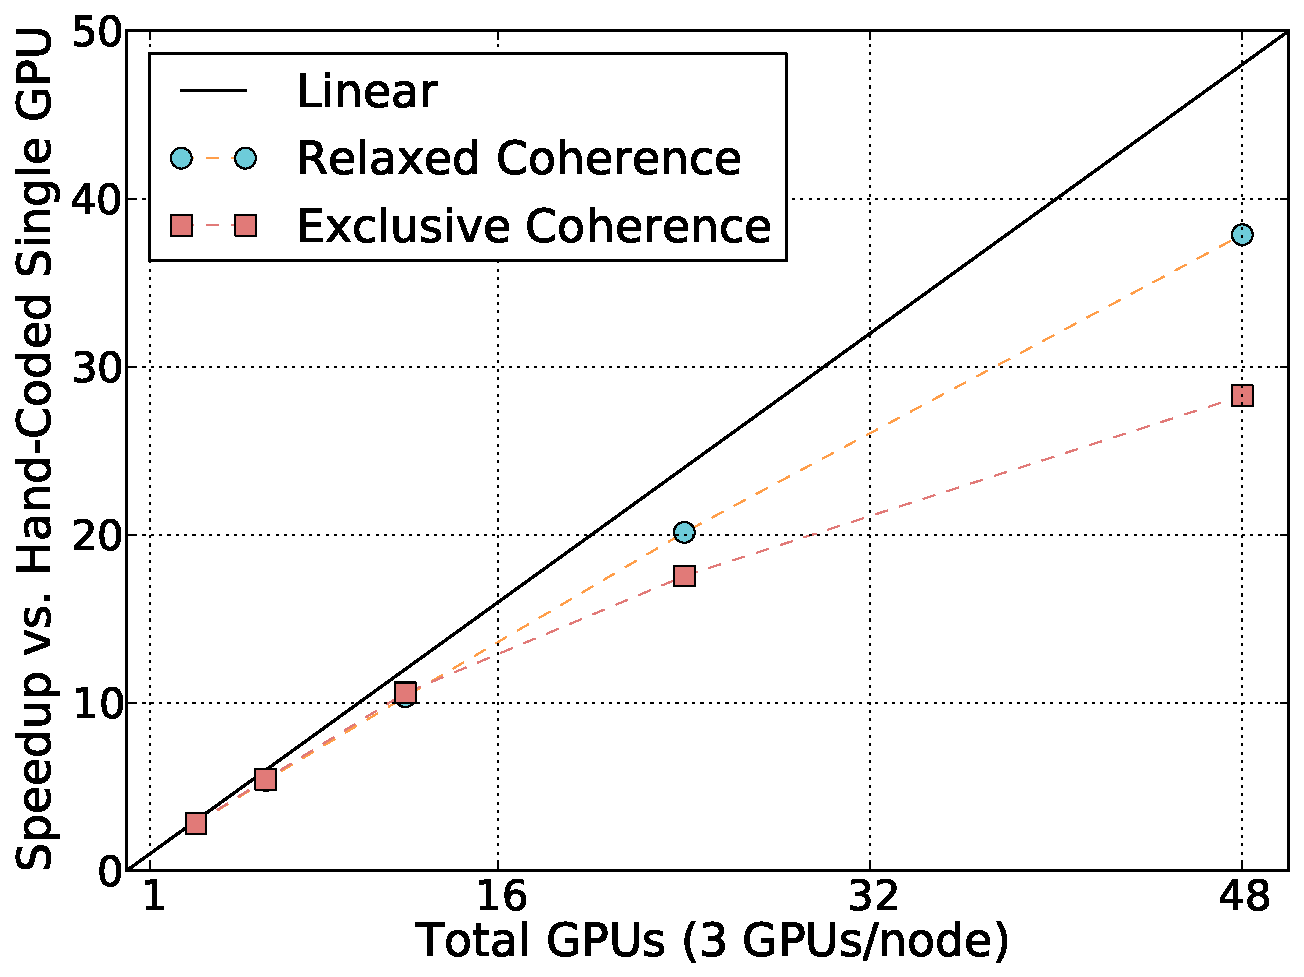
\includegraphics[scale=0.18]{figs/circuit_coherence_48.pdf}
\label{fig:circuit_excl_48}
}
\subfigure[96 Piece Problem Size]
{
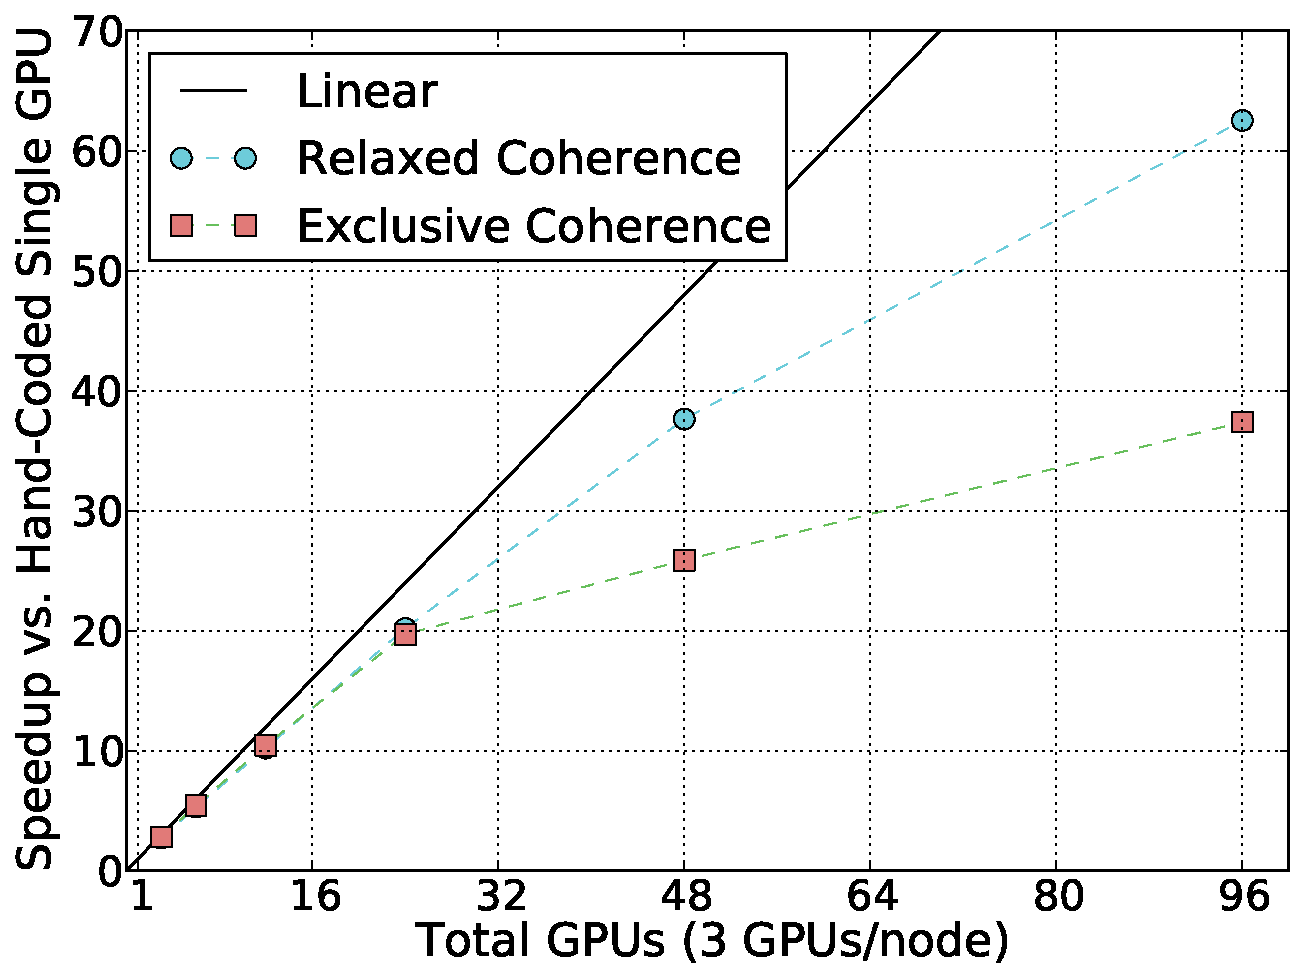
\includegraphics[scale=0.18]{figs/circuit_coherence_96.pdf}
\label{fig:circuit_excl_96}
}
\end{center}
\vspace{-4mm}
\caption{Performance of relaxed coherence modes.\label{fig:circuit_excl}}
\vspace{-6mm}
\end{figure}
%\begin{figure}
%\begin{center}
%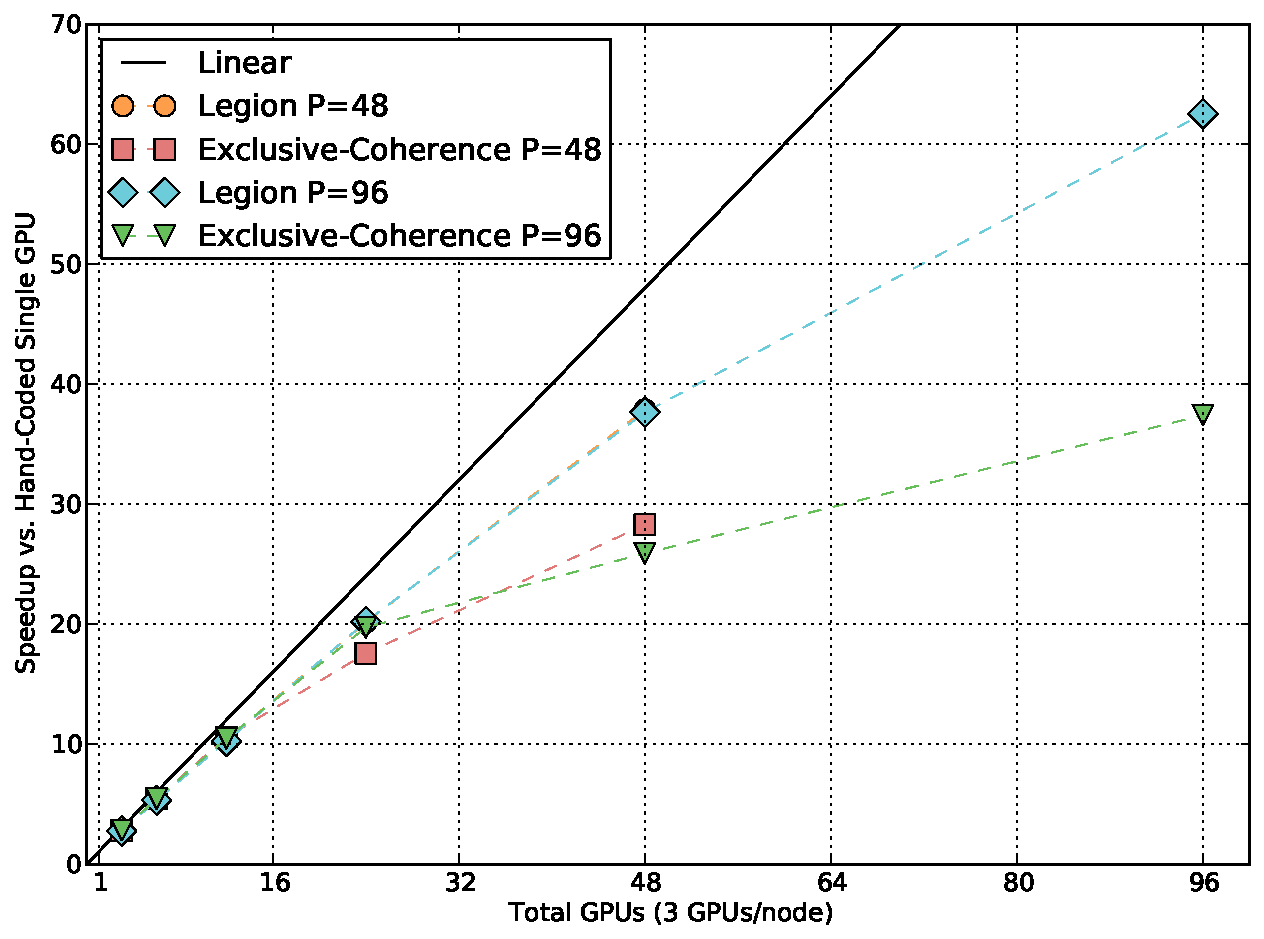
\includegraphics[scale=0.33]{figs/circuit_coherence.pdf}
%\end{center}
%\vspace{-2mm}
%\caption{Performance gains from relaxed coherence modes.\label{fig:circuit_excl}}
%\vspace{-6mm}
%\end{figure}

\subsection{Performance}
\label{subsec:relaxedperf}

To demonstrate the benefit of relaxed coherence modes, we modified the circuit example from Section~\ref{sec:example}
to use exclusive coherence instead of atomic coherence in the {\em distribute\_charge} task and compared 
the performance of the two versions.
The results are shown in Figure~\ref{fig:circuit_excl}.  Slow-downs ranged from 34\% on 48-GPUs to 67\% on 
96 GPUs and more importantly scaled with node count.  This is a direct consequence of Amdahl's Law.  
Even though the {\em distribute\_charge} tasks are a small fraction of the total work, the serialization 
that results from requiring exclusive access to the 
overlapping ghost regions limits the scalability of the application.  Relaxed coherence modes will be 
imperative for enabling the scalability of applications with aliased data on distributed memory machines.



